\documentclass[12pt]{article}
\usepackage{geometry}
\usepackage{amsfonts, epsfig}
\usepackage{amsmath}
\usepackage{wrapfig} % for wrapping text around figures and tables
\usepackage{graphicx}
\usepackage{float}
\usepackage{multirow}
\usepackage{fancyhdr}
\usepackage{booktabs} % for better table rules
\usepackage{caption} % to customize caption format
\usepackage{linegoal} % for determining the remaining width of the line
\usepackage[backend=biber, sorting=none]{biblatex}
\usepackage{subcaption}

% reference file
\addbibresource{report.bib}

\geometry{
    left=20mm,
    right=20mm,
    top=20mm,
    bottom=20mm
}

% header and footer
\makeatletter
\def\@oddhead{\parbox{\textwidth}{\raggedright\sffamily\underline{Question 1 - Visualization and analysis of the Palmer penguin dataset} \hfill \thepage}}
\def\@oddfoot{\parbox{\textwidth}{\raggedright\footnotesize\texttt{emamtm0067.github.io} / \texttt{ematm0044.github.io}}}
\makeatother

% Redefine the table and figure formats to bold
% \captionsetup[table]{labelfont=bf}
\captionsetup[table]{labelfont=bf, justification=centering}
% \captionsetup[figure]{labelfont=bf}
\captionsetup[figure]{labelfont=bf, justification=centering}
\captionsetup{font=small}

\begin{document}
\begin{center}
\subsection*{Q1 - Visualization and analysis of the Palmer dataset}
\end{center}

\begin{wraptable}{r}{0.5\textwidth} % {alignment}{width}
  \small
  \begin{center}
  \vspace{-1.5\baselineskip} % Remove space before the table
  \setlength{\abovecaptionskip}{5pt}
  \setlength{\belowcaptionskip}{5pt}
  \fontsize{10}{10}\selectfont % Change font size here
  \begin{tabular}{l|l|l}
  Attribute&Type&Values in the dataset\\
  \hline
  species&categorial&Adelie, Chinstrap, Gentoo\\
  island&categorial&Torgersen, Biscoe, Dream\\
  bill length&numerical&32.1mm - 59.6mm\\
  bill depth&numerical&13.1mm - 21.5mm\\
  flipper length&numerical&172mm - 231mm\\
  body mass&numerical&2700g - 6300g\\
  sex&categorial&Male, Female
  \end{tabular}
  \vspace{-1.5\baselineskip} % Remove space before title
  \end{center} 
  \caption{Attributes of the Palmer penguin dataset}
  \vspace{-1\baselineskip} % Remove space after the table
  \label{tab:dataset}
\end{wraptable} 

\noindent
The Palmer penguin dataset consists of 344 records of the physical attributes of three species of penguin 
living on three islands in Antarctica (Table~\ref{tab:dataset}) \cite{PM}. 
In this report, consideration is given to data cleaning and preparation, 
the dataset is explored through visualization and analysis is carried out 
to compare the accuracy performances of a small number of AI approaches. 

\vspace{\baselineskip}
\subsection*{Data cleaning - missing values, encoding, standardization and imbalance}

\begin{wrapfigure}{r}{0.5\textwidth} % {alignment}{width}
  \centering
  \vspace{-0.5\baselineskip} % Remove space before the table
  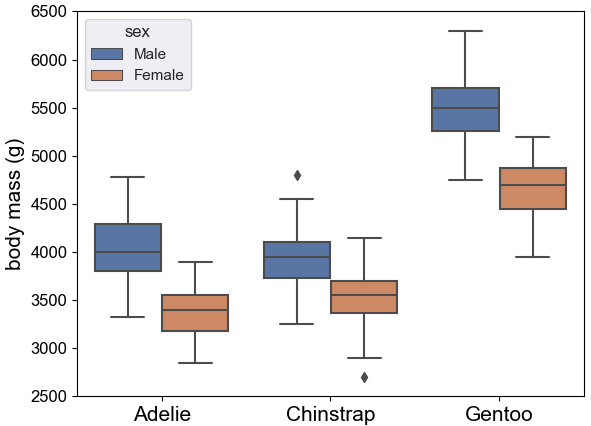
\includegraphics[width=0.48\textwidth]{sex.png} % Adjust the width as needed
  \vspace{-0.5\baselineskip} % Remove space before title
  \caption{All numerical measures show a significant statistical difference between male and female, 
  as seen in the body mass boxplot above. Shown are median values, upper and lower quartiles, 
  and outliers.}
  \vspace{-0.5\baselineskip} % Remove space before title
  \label{fig:sex}
\end{wrapfigure}   

Two records can be deleted as they are missing all numerical attributes and the sex feature, so 
any imputation is unlikely to be reliable. 
The remaining nine records are missing only the sex attribute. Figure~\ref{fig:sex} shows the physical 
attributes of the male and female of each species differ statistically and so it is reasonable to 
consider imputing a sex to those records. Following standardization, 
a Shapiro-Wilk test confirmed each numerical attribute has a normal distribution \cite{shapiro1965analysis} 
and Z-tests assessed the 
hypotheses that the missing sex value is male and that it is female \cite{freedman2007statistics}. 
Two of the records could be imputed as male and three as female 
and these were then retained in the dataset. 
The remaining four records were removed from the dataset. 
The cleaned dataset has 338 recods, 147 Adelie  
(74 male, 73 female), 68 Chinstrap (34 male, 34 female) and 123 Gentoo  (62 male, 61 female).

The random forest method is able to deal directly with the categorical features in the dataset, 
otherwise they were encoded. `One-shot' encoding was implemented, but not found to improve performance. 
A number of AI methods are known to favour numerical features 
with smaller standard deviations \cite{hastie2009elements}. 
This bias can be reduced by standardization to give zero mean and unity standard deviation. 
Standardization statistics are calculated from the training set, but are also applied to the test set. 


If a dataset is imbalanced, 
AI predictions may be biased towards classes more frequently found in the training data. 
In the Palmer penguin dataset, the number of Chinstrap records is around half of that of both Adelie and Gentoo.
However, all the methods adopted in the current work are known to be little affected by 
imbalanced data \cite{he2009learning} and so no modifications were made.

% \vspace{\baselineskip}
\subsection*{Visualization of the dataset}

Figure~\ref{fig:islands} shows the species distribution for the islands. 
Chinstrap and Gentoo penguins are found only on one island, making island a potential confounding factor whose 
individual environmental factors may influence physical characteristics. 
A Shapiro-Wilk test confirmed the normal distribution of the numerical features of the Adelie penguins (found on 
all islands) and an ANOVA test confirmed the features are not significantly influenced by the island inhabited. 
Consequently, the island is not a confounding factor in the dataset.

\begin{wrapfigure}{R}{0.5\textwidth} % {alignment}{width}
  \centering
  \vspace{-1.5\baselineskip} % Remove space before the table
  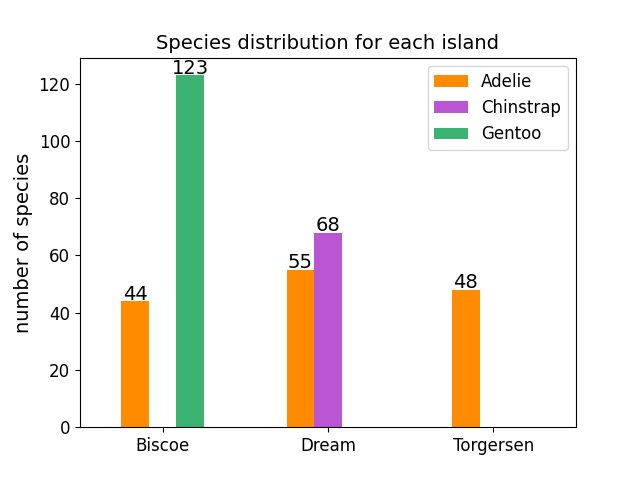
\includegraphics[width=0.48\textwidth]{islands.png} % Adjust the width as needed
  \vspace{-0.5\baselineskip} % Remove space before title
  \caption{Adelie samples are from all three islands, but Gentoo and Chinstrap from only one}
  \vspace{-1.5\baselineskip} % Remove space after title
  \label{fig:islands}
\end{wrapfigure}

Pairwise scatterplots for the numerical features are shown in Figure~\ref{fig:pairwise}. 
Bill depth, in combination with either flipper length or body mass, 
yields a separable cluster of Gentoo penguins (shown in green) allowing them to be identified. 
No pairwise combination completely separates Adelie (orange) from Chinstrap (purple) clusters, 
but the best candidate feature for doing so is in the distributions involving bill length.

Figure~\ref{fig:sex} above shows there is a difference in the body masses of the male and female samples for each of the three species. 
Differences between the sexes for the other three numerical physical characteristics in the dataset were also apparent. 
Since narrower distributions are apparent if the sex of the species is considered rather than just the species itself, 
including sex is likely to provide a finer grained distinction for species classification 
and this knowledge can be used to improve performance, as discussed in the analysis section below. 

\subsection*{Methodology}

\begin{wrapfigure}{r}{0.6\textwidth} % {alignment}{width}
  \centering
  \vspace{-3\baselineskip} % Remove space before the table
  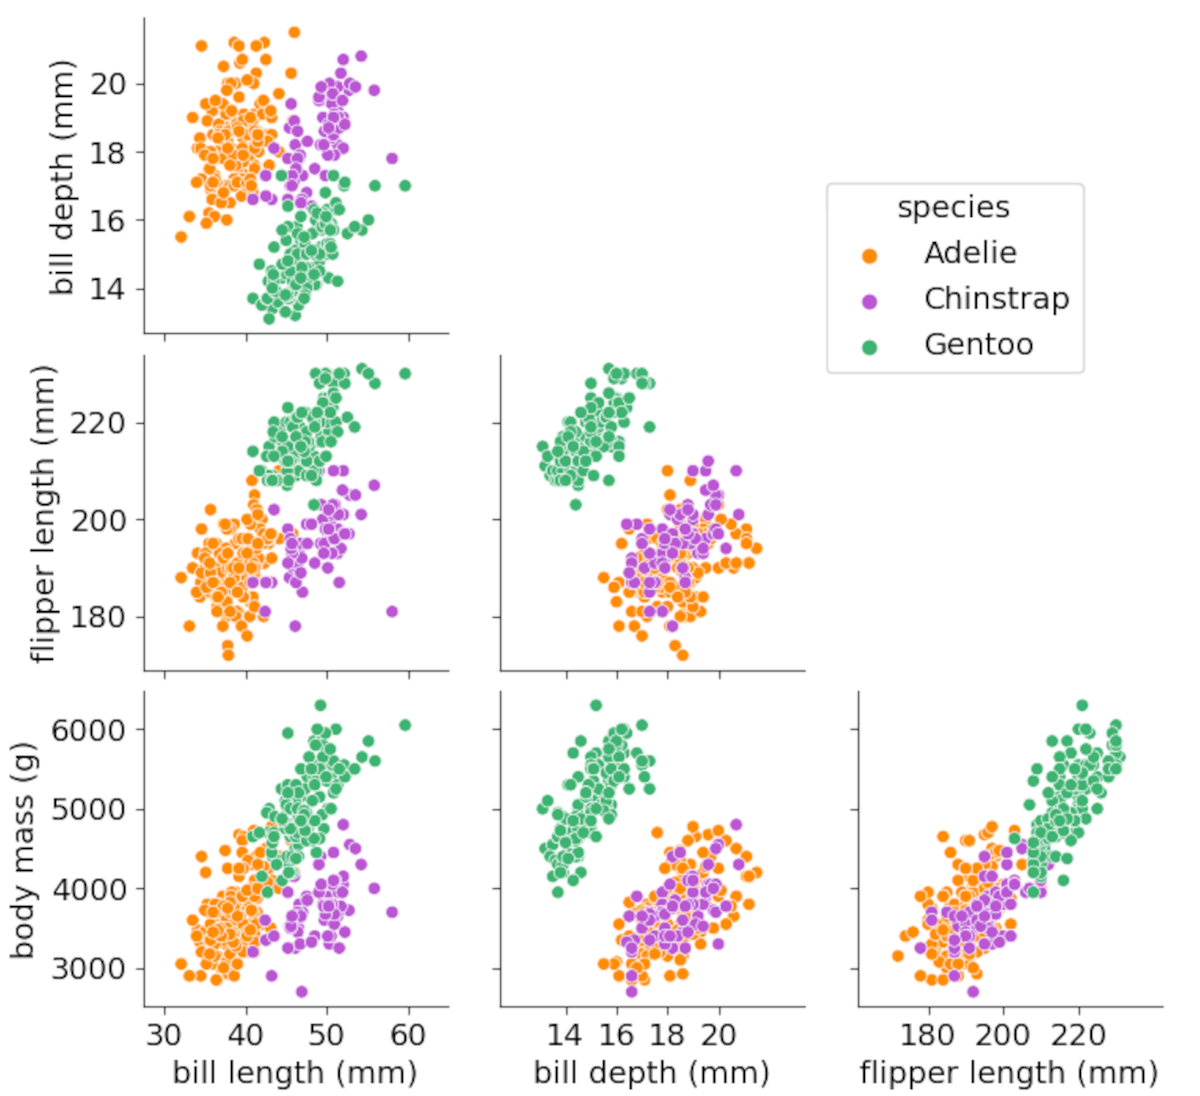
\includegraphics[width=0.58\textwidth]{pairwise.png} % Adjust the width as needed
  \vspace{-0.5\baselineskip} % Remove space before title
  \caption{Pairwise distributions of numerical features. Gentoo can be distinguished from the other species, 
  but Adelie and Chinstrap samples may not be completely separable from one another}
  \vspace{-0.5\baselineskip} % Remove space before title
  \label{fig:pairwise}
\end{wrapfigure}

All code is in Python 3.11 \cite{python311} using ‘Scikit-Learn’ libraries \cite{scikit-learn} 
under Ubuntu Linux \cite{ubuntu}. The code is available in a Gitub repository \cite{TimAIRepo}. 
Predicting the penguin species from the given features is a classification problem. 
Results are obtained from a baseline method, two convention classification approaches, 
namely \textit{k}-Nearest Neighbour (\textit{k}nn) \cite{bishop2006pattern} and random forest \cite{breiman2001random}, 
unsupervised \textit{k}-means (following cluster labelling) \cite{tan2005introduction} 
and a novel combined visualization and analysis (CVA) approach that uses 
practical visualizations and Support Vector Machine (SVM) classification.

To reduce the potential for overfitting, the classification methods (all but \textit{k}-means) were trained using 
`holdout validation', where 80\% of the dataset was used in a five-fold cross-validation 
configuration \cite{james2013introduction}. The remaining 20\% was kept for a test set. For all methods, 
the Scikit-Learn function GridSearchCV was employed to tune metaparameters \cite{scikit-learn}. 
Table~\ref{tab:metaparameters} shows the values selected for the metaparameter grid. Those giving the best 
performance were selected to generate the accuracy results from the test set. 
Scikit-Learn provides pseudo-random procedures for selecting validation and test set values and 100 of these were used 
both when selecting metaparameters and when deriving accuracy results.

\begin{wraptable}{r}{0.65\textwidth} % {alignment}{width}
  \small
  \begin{center}
  \vspace{-1.5\baselineskip} % Remove space before the table
  \setlength{\abovecaptionskip}{5pt}
  \setlength{\belowcaptionskip}{5pt}
  \fontsize{10}{10}\selectfont % Change font size here
  \begin{tabular}{l|l|l}
  Method & Metaparameters & Values considered\\
  \hline
  \multirow{3}{*}{\textit{k}nn} & number of nearest neighbours \textit{k}	  & \textit{\textbf{1}}, 2, 3, 4, 5, 6, 8, 10 \\
                            & weight function for prediction	& \textit{\textbf{uniform}}, distance \\
                        & distance metric for neighbours	& \textbf{Manhattan}, Euclidean \\
  \hline
  \multirow{5}{*}{random forest} & number of trees in the forest & 5, \textit{textbf{10}}, 15, 20, 25 \\
                                 & maximum depth of trees	         & \textit{\textbf{no maximum}}, 10, 20 \\
                                 & minimum samples to split node	 & \textit{\textbf{2}}, 5, 10 \\
                                 & minimum samples at leaf node    & \textit{\textbf{1}}, 2, 4 \\
                                 & function for quality of split   & \textit{\textbf{gini}}, entropy \\
  \hline
  \multirow{4}{*}{\textit{k}-means} & number of clusters \textit{k}  & 2, \textit{\textbf{3}}, 4, 5, 6, 7, 8, 9, 10 \\
                              & centroid initialization method         & \textit{\textbf{k-means++}}, random \\
                              & number of runs for centroid seeds	     & 2, \textit{\textbf{5}}, 10, 20 \\
                              & maximum number of iterations           & 5, \textit{\textbf{10}}, 20, 50 \\
  \hline
    \multirow{3}{*}{CVA} & regularization parameter (C)  & 0.1, 1, \textit{\textbf{10}}, 100 \\
                          & kernel coefficient (gamma)   & \textit{\textbf{1}}, 0.1, 0.01, 0.001 \\
                          & kernel type                  & rbf, \textit{\textbf{linear}}, polynomial \\
  \hline
  \end{tabular}
  \vspace{-1.5\baselineskip} % Remove space before title
  \end{center} 
  \caption{Metaparameters considered in training. 
  The values shown in italics most consistently produced results of 
  best accuracy during validation and were selected for generating results}
  \vspace{-1\baselineskip} % Remove space after the table
  \label{tab:metaparameters}
\end{wraptable} 

\subsection*{Results and analysis}

The results in Table~\ref{tab:results} include a baseline that is used to demonstrate performance improvements achieved by the AI methods being considered. 
In classification, the baseline method is often simply to select the most frequent class in the observations and, 
in this work, this is the Adelie penguins, giving an accuracy of 43.49\% (147/338).

\begin{wraptable}{r}{0.6\textwidth} % {alignment}{width}
  \small
  \begin{center}
  \vspace{0\baselineskip} % Remove space before the table
  \setlength{\abovecaptionskip}{5pt}
  \setlength{\belowcaptionskip}{5pt}
  \fontsize{10}{10}\selectfont % Change font size here
  \begin{tabular}{l|l}
  Method & Accuracy\\
  \hline
  baseline, most numerous species & 43.49\% \\
  \hline
  \textit{k}NN, all features	& 99.24\% \\
  \textit{k}NN, no island &	99.46\% \\
  \hline
  random forest, all features	& 98.57\% \\
  random forest, no island, flipper length or body mass	& 98.57\% \\
  \hline
  \textit{k}-means, all numerical features & 97.06\% \\
  \textit{k}-means, separate clusters for each sex & 98.23\% \\
  \hline
  CVA using bill depth, flipper length, bill length	& 98.56\% \\
  CVA using bill depth, flipper length, bill length, sex &98.78\% \\
  \hline
  \end{tabular}
  \vspace{-1.5\baselineskip} % Remove space before title
  \end{center} 
  \caption{Mean classification accuracy from 100 test sets each generated by a pseudo random approach 
  and using the parameters identified in Table~\ref{tab:metaparameters}}
  \vspace{-2\baselineskip} % Remove space after the table
  \label{tab:results}
\end{wraptable} 

\textbf{Classification method 1 - \textit{k}nn}  
The performance of \textit{k}nn was found to be improved by omitting features from training. 
An exhaustive search involving omitting all combinations of features in turn determined that the best accuracy was obtained 
when island was omitted and this occurred when \textit{k}=3. It appears that island was not providing any additional information 
and the higher value of \textit{k} implies better generalization may have been achieved.

\textbf{Classification method 2 - Random forest}  
Including all of the features in the analysis provided an accuracy marginally better 
than could be achieved using \textit{k}nn when its features were carefully selected. 
No performance improvement was found by using fewer features, indicating that 
considerably less implementation effort is needed to achieve good performance using random forest. 
A marginal improvement in performance was apparent when island, flipper length or body mass were not included in training.

\begin{wrapfigure}{r}{0.5\textwidth} % {alignment}{width}
  \centering
  \vspace{-0.5\baselineskip} % Remove space before the table
  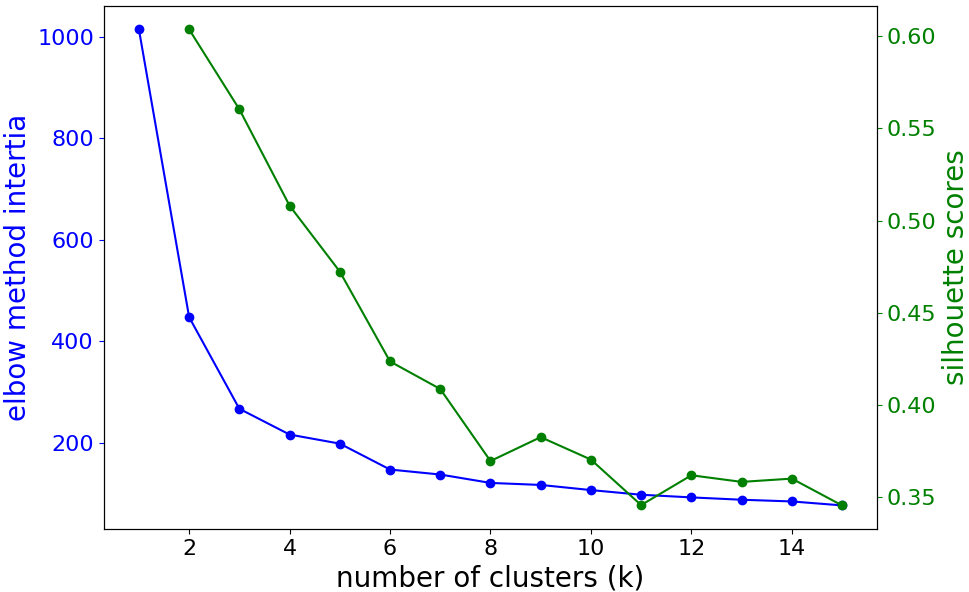
\includegraphics[width=0.48\textwidth]{kmeansvalue.png} % Adjust the width as needed
  \vspace{-0.5\baselineskip} % Remove space before title
  \caption{To estimate k for \textit{k}-means, the elbow method uses the change in slope of `inertia' 
  (here \textit{k}=3) and the silhouette method uses the score closest to 1 (here \textit{k}=2)}
  \vspace{-0.5\baselineskip} % Remove space before title
  \label{fig:kmeansvalue}
\end{wrapfigure}

\textbf{Unsupervised method - \textit{k}-means}  
Although an unsupervised clustering method, 
\textit{k}-means can be used for classification by matching clusters to classes. 
The \textit{k}-means method is normally applied only to numerical features so only they were included in this work. 
The number of clusters (\textit{k}) can be selected using elbow and silhouette methods, 
as shown in Figure~\ref{fig:kmeansvalue}. Empirically, accuracy improved significantly when \textit{k}>3 
as clusters were not reliably formed for all three species for smaller values of \textit{k},  
Figure~\ref{fig:kmeansmap} illustrates the mapping of classes to clusters for two feature dimensions. 
No improvement in accuracy was obtained by reducing the number of features, 
but, in an additional experiment, a set of \textit{k}-means clusters was created for each sex 
and this led to a small improvement in accuracy. 

\begin{wrapfigure}{r}{0.5\textwidth} % {alignment}{width}
  \centering
  \vspace{-0.5\baselineskip} % Remove space before the table
  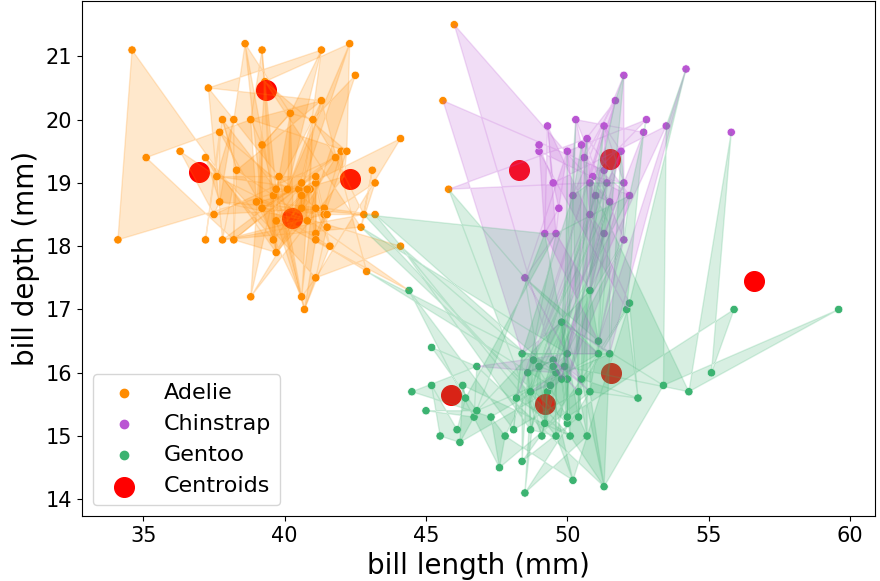
\includegraphics[width=0.48\textwidth]{kmeansmap.png} % Adjust the width as needed
  \vspace{-0.5\baselineskip} % Remove space before title
  \caption{\textit{k}-means clusters mapped to species according to majority voting. 
  Assignments to classes are shown by polygon colours (here \textit{k}=10 and colouring limited to 50 samples).}
  \vspace{-0.5\baselineskip} % Remove space before title
  \label{fig:kmeansmap}
\end{wrapfigure}

\textbf{A novel combined visualization and analysis (CVA) approach}  
This work introduces the CVA approach that visualizes pairwise combinations of numerical data 
to identify a short sequence of two-dimensional SVM classifiers. 
CVA requires manual effort to understanding the nature of the dataset, 
in contrast with `black box' classification approaches that are applied with limited knowledge 
of the method and little insight into the nature of the data. 
The drawbacks of the CVA approach are that it may not always be feasible to extract the necessary insights 
from visualizations and that it becomes more difficult to apply as the number of features is increased. 
In application to the Penguin data, CVA was able to produce results of accuracy almost as good 
as conventional approaches.

An application of CVA to the Penguin dataset is illustrated in Figure~\ref{fig:CVA}. 
Figure~\ref{fig:CVA_part_a} shows the relationship between bill depth and flipper length and 
SVM is used to find a suitable `decision boundary' that separates Gentoo from the other two species. 
Figure~\ref{fig:CVA_part_b} then shows a second SVM line that best separates Adelie and Chinstrap using bill length and bill depth. 
A small improvement in accuracy was achieved when two separate SVM models were developed, one for each penguin sex.

\begin{figure}[!ht]
  \begin{subfigure}{0.5\textwidth}
    \centering
    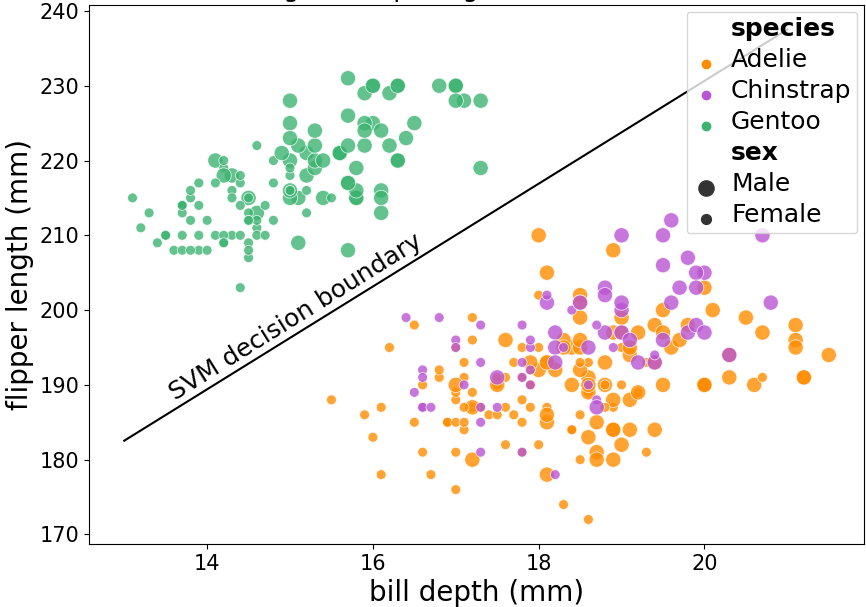
\includegraphics[width=1.05\textwidth]{sup_fliplen_billdepth.png} % Adjust the width as needed
    \caption{bill depth and flipper length with a decision boudary to distinguish Gentoo from the other two species}
    \label{fig:CVA_part_a}
  \end{subfigure}
  \hfill
  \begin{subfigure}{0.5\textwidth}
    \centering
    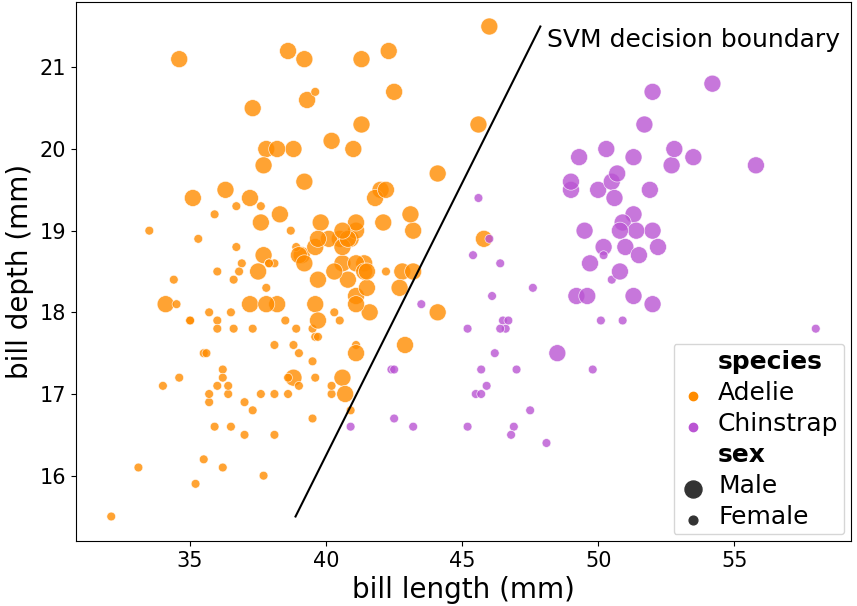
\includegraphics[width=1.05\textwidth]{sup_billlen_billdepth.png} % Adjust the width as needed
    \caption{bill length and bill depth allow the Adelie and Chinstrap species to be distingushed from one another}
    \label{fig:CVA_part_b}
  \end{subfigure}
  \caption{Example of two-stages CVA approach applied to the Palmer penguin data. 
  The two-dimensional lines of separation shown in the figures are fitted using SVM 
  and only to training data for the features shown on the axes.}
  \label{fig:CVA}
\end{figure}

\subsection*{Conclusions}

With careful data preparation, optimization of metaparameters and robust application of training and testing methods, 
the \textit{k}nn and random forest classification methods produced high-quality results. 
The \textit{k}-means classification accuracy results were somewhat worse, 
but this is to be expected as the approach does not take advantage of target data information that is known to the supervised approaches. 

A classifier that is able to achieve 100\% accuracy for the given data is possible, 
but its performance when applied to new unseen data would likely exhibit poor generalization.
The novel CVA approach is designed to use insights available in visualizations. 
Although needing to be tailored to each problem and not well-suited to high-dimensionality data, 
its internal operations are easy to visualize, an advantage not afforded to general-purpose classification methods. 
For the penguin data, it was able to produce accuracy results similar to those of other classification methods. 

\printbibliography


\end{document}
